% Latex课程报告模板 袁老师封皮
 
\documentclass{article}
\usepackage[UTF8,zihao=-4]{ctex}
\usepackage{amsfonts} 
\usepackage{amsmath} 

\usepackage[top=2.54cm, bottom=2.54cm, left=3.18cm, right=3.18cm]{geometry}
\geometry{paper=a4paper}
\usepackage{graphicx}
\usepackage{gbt7714}
\usepackage{setspace}
\usepackage{indentfirst}
\usepackage{titlesec}
\usepackage{fancyhdr}    

\newcommand{\triangleq}{\stackrel{\mathrm{def}}{=}} 

\newCJKfontfamily\heititext{SimHei}[
  Path = C:/Windows/Fonts/,  % Windows字体目录
  AutoFakeBold = 2,        % 加粗强度(3.5为最佳视觉效果)
]


\newCJKfontfamily\simsuntext{SimSun}[
  Path = C:/Windows/Fonts/,  % Windows字体目录
  AutoFakeBold = 2,        % 加粗强度(3.5为最佳视觉效果)
]

\newCJKfontfamily\hwtext{STXinwei}[
  Path = C:/Windows/Fonts/,  % Windows字体目录
  AutoFakeBold = 2,        % 加粗强度(3.5为最佳视觉效果)
]

\begin{document}
% 自定义变量
\newcommand{\TITLE}{无人机辅助通信系统中的轨迹设计与资源分配算法} %标题
\newcommand{\AUTHOR}{周卓} %作者
\newcommand{\STUDENTNO}{2240201012} %学号

\newcommand{\sizethirty}{\fontsize{30pt}{50pt}}  % 30号字(初号)

% 行距与缩进
\onehalfspacing
\setlength{\parindent}{2em}

% 自定义各级标题格式字体
\titleformat{\section}
  {\heititext \zihao{3} \bfseries \centering}
  {\thesection}
  {1em}{}
\titlespacing{\section}{0pt}{24pt}{18pt}

\titleformat{\subsection}
  {\simsuntext \zihao{4} \bfseries \raggedright}
  {\thesubsection}
  {1em}{}
\titlespacing{\subsection}{0pt}{18pt}{12pt}

\titleformat{\subsubsection}
  {\simsuntext \zihao{-4} \bfseries \raggedright}
  {\thesubsubsection}
  {1em}{}
\titlespacing{\subsubsection}{0pt}{12pt}{6pt}

%%%%%%%%%%%%% 封面页 %%%%%%%%%%%%

\pagestyle{empty}
\begin{flushright}
{
     {\simsuntext \zihao{-4} \bfseries 2024-2025学年第二学期}
    
}
\end{flushright}


\begin{figure}[h]
    \centering
    
\includegraphics[width=0.8\textwidth]{./城院logo3.png}
    % \caption{}
\end{figure}
% \vspace*{12em}
\begin{center}
    {\hwtext\bfseries\sizethirty 
    《现代无线与移动通信系统》\\[1.5\baselineskip]  % 手动调整行距
    课程报告}
\end{center}
\begin{figure}[h]
    \centering
    
\includegraphics[width=0.33\textwidth]{./城院logo2.png}
    % \caption{}
\end{figure}
% \vspace{3em}

\newcommand{\fssi}{\fangsong\zihao{4}}

\begin{center}
{ \fssi % 这里的字号也可以用别的方式修改

\makebox[4em][s]{姓名}:\hspace{1em}\underline{\makebox[14em][c]{\AUTHOR}}\\
\vspace{1em}
\makebox[4em][s]{学号}:\hspace{1em}\underline{\makebox[14em][c]{\STUDENTNO}}\\
\vspace{1em}
\makebox[4em][s]{专业班级}:\hspace{1em}\underline{\makebox[14em][c]{电子信息2402}}\\
\vspace{1em}
\makebox[4em][s]{所在学院}:\hspace{1em}\underline{\makebox[14em][c]{信息与电气工程学院}}\\
\vspace{1em}
\makebox[4em][s]{指导老师}:\hspace{1em}\underline{\makebox[14em][c]{袁 建 涛}}\\
\vspace{1em}
\makebox[4em][s]{日期}:\hspace{1em}\underline{\makebox[14em][c]{2025.4.16}}\\
}
\end{center}



%%%%%%%%%%%%% 标题 摘要 %%%%%%%%%%%%



\title{\TITLE}
% \author{\AUTHOR~ \STUDENTNO}
\date{}
\maketitle

\thispagestyle{empty}

\begin{center}
  {\heititext\zihao{3}\bfseries 摘要}  % 标题加粗
\end{center}
\vspace{0.5em}
{
    \simsuntext\zihao{-4}\linespread{1.5}\selectfont
    \hspace{2em}无人机辅助通信作为6G网络的关键技术,通过三维机动能力显著提升通信覆盖质量与感知精度,为解决传统地面基站部署受限和频谱资源紧张问题提供了创新方案。本文介绍单无人机辅助的多用户下行通信系统,其中无人机配备多天  线和雷达,能够利用雷达探测地面用户的位置。为了降低导频开销,使用了一种基于深度强化学习的算法,利用雷达探测  的用户初始位置预测其未来的运动轨迹。基于此预测,通过联合优化无人机轨  迹和预编码矩阵,旨在最大化一段时间内所有用户的通信速率和。构建了集成通感一体化(ISAC)技术的双时间尺度优化框架:在短时间尺度上动态调整预编码矩阵以抑制多用户干扰,在长时间尺度上优化无人机悬停位置以降低移动能耗。系统模型采用均匀平面阵列天线与自由空间路径损耗信道,通过雷达信号实时感知用户位置,并建立包含用户移动特征的马尔可夫决策过程。
    \par  % 确保行距生效
    \vspace{0.5em}
    \noindent{\simsuntext\zihao{-4}\bfseries 关键词:} \simsuntext\zihao{-4}无人机辅助通信;无人机轨迹设计;强化学习;
}

%%%%%%%%%%%%% 目录 %%%%%%%%%%%%

\newpage
\pagestyle{plain}
\pagenumbering{roman}
\tableofcontents

%%%%%%%%%%%%% 正文 %%%%%%%%%%%%

\newpage
\pagestyle{fancy}
\fancyhf{}               % 清空默认页眉页脚
\renewcommand{\headrulewidth}{0pt} % 取消页眉线
\pagenumbering{arabic} \setcounter{page}{1} % 重置为阿拉伯数字
\cfoot{第 \thepage\ 页 \hspace{0.5em} 共 \pageref{EndBody} 页}

\section{技术综述}
    \subsection{无人机辅助通信概述}
    无人机辅助通信作为6G网络的重要组成部分和关键技术,近年来受到学术界和工业界的广泛关注\cite{mishra2022drone}。该技术通过搭载无线通信模块的无人机平台,能够快速部署到传统地面基站难以覆盖的区域,特别是在应急通信、灾害救援和军事应用等场景中展现出显著优势。相较于传统地面通信系统,无人机辅助通信具有三大核心优势:首先,在部署效率方面,无人机系统能够在无固定基础设施条件下实现分钟级快速部署,克服了地面基站建设周期长、受地理条件限制的缺陷;其次,在通信质量方面,无人机通过空中机动可以显著提高视距(LOS)通信概率,有效规避建筑物和地形遮挡导致的小尺度衰落和阴影衰落问题,使通信可靠性提升15-20dB;最后,在网络灵活性方面,基于智能算法的动态路径规划技术使无人机能够根据实时需求调整飞行高度和覆盖范围,支持1000+终端/km²的高密度连接,其能效比较传统基站提升30-50\%。当前技术发展正朝着智能反射面集成、毫米波空口设计和数字孪生网络优化等方向快速演进,为6G时代的全域覆盖和智能组网提供关键支撑。

    相较于5G网络,6G的核心特征和主要愿景之一是实现更高层次的智能化,这使得人工智能(AI)技术成为6G建设中的关键使能要素。近年来,得益于计算能力的显著提升、深度学习算法的持续优化以及大数据技术的快速发展,AI技术已在自动驾驶、计算机视觉和远程医疗等多个领域取得突破性进展\cite{patel2007applications},并正在重塑移动通信系统的架构与运行范式。特别是在无人机辅助通信领域,AI技术通过实时信道状态分析、智能资源调度和自主轨迹规划,能够动态优化无人机网络的拓扑结构和传输参数,显著提升系统的频谱效率、能量效率和通信可靠性。基于深度强化学习的自主决策系统可以实时处理多维环境信息,实现毫秒级的飞行路径调整和资源分配,从而有效应对复杂无线环境下的干扰管理和负载均衡挑战,为6G网络提供高度自适应的三维立体覆盖能力。


    
    \subsection{通感一体化技术概述}

    6G通信网络的演进正推动机器类通信、自动驾驶和扩展现实等智能应用从理论走向实践,这些新兴应用对数据传输速率和传感精度提出了前所未有的严苛要求。传统通信与传感分离的设计架构已难以满足高吞吐量传输与高精度感知的协同需求,成为制约智能应用发展的关键瓶颈。与此同时,全球无线通信需求的爆发式增长使得频谱资源日益稀缺,尤其在物联网和大规模机器类通信场景下,传统静态频谱分配模式已无法适应未来高密度、高效率的通信需求。这一背景促使通感一体化(ISAC)技术成为6G网络研究的核心方向\cite{wei2023integrated},其通过深度整合通信与感知功能,实现频谱资源的动态复用与优化配置。

    为应对这一技术挑战,雷达与通信频谱共享(RCSS)技术应运而生并受到广泛关注\cite{liu2020radar}。RCSS研究主要聚焦于两大技术路径:雷达通信共存(RCC)系统和双功能雷达通信(DFRC)系统。RCC系统通过频谱共享机制使雷达与通信设备协同工作,采用动态干扰管理技术来缓解系统间干扰,但其独立运行的特性导致协同效率受限。DFRC系统则通过硬件架构重构和波形联合设计,实现通信与雷达感知的深度集成,不仅将频谱效率提升30\%以上,还显著降低了系统复杂度和部署成本\cite{ma2020automotive},为ISAC技术的工程化应用奠定了重要基础。
    
    值得注意的是,ISAC技术性能高度依赖于收发端与目标之间的视距传播条件。在复杂地理环境中,无人机凭借其三维机动能力可动态优化飞行轨迹,将视距通信概率提升至85\%以上\cite{zhu2024enabling}。通过将无人机平台与ISAC技术深度融合,不仅能够突破传统地面系统的覆盖限制,还能实现通信速率与感知精度的协同提升,为6G网络构建具备环境自适应能力的智能通信感知一体化体系。这种创新架构通过实时信道状态感知和智能资源调度,可支持10Gbps级数据传输与厘米级定位精度的同步实现,为自动驾驶、工业物联网等关键应用提供可靠的技术支撑。

    \subsection{预编码技术概述}

    在多天线通信系统中,天线单元间的相互干扰和信号传输过程中的功率衰减问题,往往导致未经处理的发射信号在接收端出现严重的信号质量劣化,进而直接影响通信系统的整体性能表现。为解决这一关键技术难题,预编码技术作为一种高效的信号预处理方法,在现代无线通信领域特别是多输入多输出(Multiple-Input Multiple-Output, MIMO)系统中得到了深入研究和广泛应用\cite{ye2003optimized}。该技术的核心原理在于:发射端基于实时获取的信道状态信息(Channel State Information, CSI),通过特定的矩阵运算算法对已调制的待发送信号进行预处理,使信号波形能够自适应匹配当前信道的传输特性,从而有效抑制多径传播引起的符号间干扰(Inter-Symbol Interference, ISI),并实现接收端信噪比(Signal-to-Noise Ratio, SNR)的最大化优化。这一技术在下行链路传输场景中具有特殊的重要性,特别是在多用户共享相同频谱资源的通信环境下,预编码技术能够智能地调整各天线的发射信号参数,确保每个用户终端都能获得最优的信号接收质量,显著提升系统的通信可靠性和传输稳定性。具体实现过程中,基站设备通过上行信道估计获取各用户设备的CSI信息,并据此动态调整发射信号的幅度和相位参数。这种基于用户个性化的信号优化处理,可以大幅降低多用户之间的同频干扰(Co-Channel Interference),即使在复杂的无线传播环境和密集的用户分布场景下,仍能保证系统维持优异的通信性能指标。

根据信号处理域的不同和实现技术路线的差异,预编码技术主要可分为三种典型实现方式:数字预编码、模拟预编码以及混合预编码\cite{busari2017millimeter}。数字预编码技术主要在数字基带域完成信号处理,通过数字信号处理器(DSP)实现精确的复数权重调整;模拟预编码技术则在射频模拟域进行信号处理,通常采用可编程相控阵列天线来实现波束方向的动态调控;而混合预编码技术创造性地结合了前两者的技术优势,通过模拟预编码模块实现粗粒度的波束成形,再借助数字预编码模块进行细粒度的干扰协调,从而达到系统性能和硬件复杂度的最佳平衡。在面向6G的演进过程中,预编码技术将持续发挥其关键作用,特别是在提升系统频谱效率、扩展网络容量极限、支持超高用户密度和实现超低时延传输等核心性能指标方面具有不可替代的价值\cite{yan2020hybrid}。随着6G网络对传输速率(峰值速率预计达1Tbps)、端到端时延(低于1ms)、通信可靠性(99.999\%以上)以及海量设备连接(每平方公里百万级连接)等方面提出更为严苛的要求,预编码技术的持续创新和深度优化将成为实现这些突破性目标的关键使能技术。一方面,6G网络将大规模部署基于超大规模天线阵列(Massive MIMO)的基站设备,这些基站可能配置数百甚至上千个天线单元来服务密集分布的用户终端,此时预编码技术能够智能优化各天线的信号传输路径,有效抑制用户间干扰,将频谱利用率提升至新的高度。另一方面,6G网络将探索利用太赫兹(Terahertz, THz)频段进行通信,虽然该频段可提供数十GHz的超大带宽资源,但其信号在传播过程中会遭受严重的路径损耗和大气吸收衰减,导致有效传输距离显著缩短。在这种情况下,预编码技术通过精确的波束赋形和能量聚焦,可以大幅降低信号在传输过程中的功率损失,从而有效提升太赫兹通信的系统覆盖能力和传输效率。

  \subsection{单无人机辅助通信系统研究现状}

  近年来,单无人机辅助通信系统凭借其灵活的移动基站特性,在无线通信领域获得了广泛研究关注。研究者们重点围绕无人机轨迹规划、预编码器设计和资源分配等关键问题展开深入优化。随着通感一体化(ISAC)技术的发展,无人机平台的高机动性优势进一步凸显,使其能够同时高效执行环境感知和无线通信双重功能。现有研究主要从以下两个技术路线展开探索:

  在传统优化算法方面,文献\cite{xu2020multiuser}针对单无人机多用户下行系统,创新性地结合单调优化理论和半正定松弛法,实现了无人机二维轨迹与预编码矩阵的联合优化,在保证全局最优解的同时,提出基于连续凸近似的低复杂度迭代方案。文献\cite{ge2020joint}通过分解优化框架,将智能反射面辅助无人机系统中的主动波束形成、被动波束形成和飞行轨迹规划问题转化为三个可并行求解的子问题,并推导出反射元件相移的闭式解。针对ISAC应用场景,文献\cite{meng2022uav}在满足感知频率和波束图约束条件下,建立了无人机轨迹、发射预编码器和感知时隙的联合优化模型;文献\cite{lyu2022joint}则通过混合凸优化方法,在功率和飞行约束下最大化用户加权和速率。文献\cite{li2020joint}创新性地将匹配理论与逐次凸优化相结合,解决了非正交多址无人机网络的能量效率优化问题。

  然而,这些基于传统优化理论的方法普遍存在计算复杂度高的问题,难以满足6G网络对实时性的严苛要求。为此,机器学习方法逐渐成为新的研究热点。文献\cite{yuan2020learning}利用深度学习预测无人机抖动导致的波束偏移,提出了自适应波束对齐方案。在强化学习方向,文献\cite{zhou2022constrained}将约束马尔可夫决策过程与柔性Actor-Critic算法相结合,实现了能量受限下的任务时间优化;文献\cite{khurshid2023drl}采用深度确定性策略梯度算法,同步优化三维部署与资源分配;文献\cite{bayerlein2020uav}通过深度双Q网络实现了吞吐量最大化与飞行时间最小化的多目标优化。文献\cite{liu2020machine}提出的衰减深度Q网络算法,在可重构智能表面辅助场景中平衡了训练效率与收敛性能。文献\cite{zhang2023deep}基于近端策略优化算法开发了无人机在线控制系统,而文献\cite{zhang2020trajectory}则引入迁移学习机制加速轨迹优化过程。

  需要特别指出的是,现有研究大多建立在用户位置已知的理想假设下,这与实际通信环境中用户动态移动的特性存在显著差距。这一局限性促使未来研究需要更加关注以下方向:1)开发具有环境自适应能力的在线学习算法;2)设计支持用户位置不确定性的鲁棒优化框架;3)探索感知-通信-计算资源的跨域协同机制。这些突破将推动无人机辅助通信系统向智能化、自适应化方向持续演进。

\section{UAV辅助通信系统模型介绍}
    \subsection{系统模型概述}
    如图\ref{Fig3-1}所示,考虑单无人机辅助的多用户下行通信系统,其中包含一架可移动的无人机和$K$个随机移动的地面用户,地面用户的集合记作$\mathcal{K}=\{1,2,\ldots,K\}$。每位用户配备单根天线,而无人机则装备了$M$根天线,组成均匀平面阵列(Uniform Planar Array,UPA),其中每行包含$M_x$根天线,每列包含$M_y$根天线,满足$M = M_x\times M_y$。无人机集成了ISAC系统,能够通过雷达信号探测地面用户的位置,以获取用户的初始位置。此外,无人机在空中悬停并提供服务,为了充分利用无人机的高机动性,其可以周期性地调整位置以优化系统性能。
    \begin{figure}[h]
      \centering
      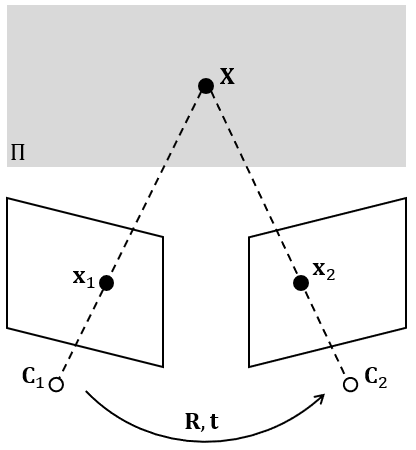
\includegraphics[width=0.5\textwidth]{wuxian/1.jpg}
      \caption{无人机辅助通信系统模型}
      \label{Fig3-1}
  \end{figure}

    随着地面用户的移动,瞬时CSI也会发生变化,为了提供稳定且高质量的通信服务,无人机可以周期性地调整自身位置。然而,由于无人机的服务范围较大,且单次用户移动对无人机位置调整的影响较小,因此频繁无人机调整位置并非高效的策略,且通常是不必要的。为了解决这一问题,引入了一种双时间尺度的方案。如图\ref{Fig3-2}所示,考虑一个长度为$T$的超帧,且在此期间信道的统计特性保持不变。在该方案中,我们定义短时间尺度为时隙,在每个时隙内优化无人机的预编码矩阵;定义长时间尺度为帧,在每个帧内优化无人机的悬停位置。具体而言,超帧被均匀划分为$T_s$个帧,每帧由$F_s$个时隙组成。因此,在整个超帧期间,时隙的总数$N$满足$N = T_s \times F_s$,且每个帧的持续时间为$\delta = \frac{T}{N}$。基于这种时间划分,在不同时间尺度下有以下假设:
    假设所有用户在每个时隙结束时改变位置,并且在每个时隙内瞬时CSI保持不变。因此,在每个时隙结束时,根据瞬时CSI更新无人机的发射预编码矩阵。
    假设无人机在一个帧内保持位置不变。当一个帧结束时,根据该帧内所有时隙的CSI优化下一个无人机服务位置,并假设无人机在下一帧开始前移动到该位置。  
    



  \begin{figure}[h]
    \centering
    \includegraphics[width=4in]{./images-p/双时间尺度.png}
    \caption{双时间尺度方案}
    \label{Fig3-2}
  \end{figure}
  
  \subsection{信道模型}\label{section3-1-3}
    为了不失一般性,采用二维笛卡尔坐标系。在空中悬停时,无人机保持固定高度$H$,其在第$t$帧的水平坐标表示为${p}[t] = [x[t], y[t]] \in \mathbb{R}^{1 \times 2}$。用户$k$在第$i$时隙的水平坐标可以表示为$\bold{q}_k[i] = [x_k[i], y_k[i]] \in \mathbb{R}^{1 \times 2}$。因此,无人机与用户$k$在第$i$时隙之间的水平距离可以表示为:
    \begin{equation}\label{eq3-1}
      d_{k,i}=\sqrt{H^2+||\bold p\left[t\right]-\bold q_k\left[i\right]||^{2}},
    \end{equation}
    其中,$||\cdot ||$表示$l_2$范数,第$i$个时隙在第$t$帧内,即$tF_s+1 \le  i \le (t+1)F_s$。\par
    一般来说,在无人机和用户之间的无线链路中,应同时考虑LoS和非视距(Non Line of Sight,NLoS)路径两部分。然而,实验证明,在无人机飞行高度足够高且地面障碍物较少的区域,LOS路径出现的概率较高\cite{matolak2015unmanned}。因此,省略了NLoS部分,仅考虑LoS路径,并采用自由空间路径损耗模型来表征LoS分量。在第$i$个时隙,无人机到用户$k$的瞬时信道可以表示为:
    \begin{equation}\label{eq3-2}
      \begin{split}
        \bold h_{k,i}&=\gamma_0d_{k,i}^{-2}\bold a^{H}_{k,i},
      \end{split}
    \end{equation}

    \noindent 其中,$\gamma_0$表示在参考距离1米处的信道功率,$\bold a^{H}(\theta_k\left[i\right],\phi_k\left[i\right]) \in \mathbb{C}^{M\times 1}$表示第$i$个时隙从无人机到用户$k$的传输天线阵列响应。它可以表示为:
    \begin{equation}\label{eq3-3}
      \begin{split}
        \bold a^{H}_{k,i}&=(1,\dots,e^{-j\pi m_x\sin{\theta_k\left[i\right]}\cos{\phi_k\left[i\right]}},\dots,e^{-j\pi(M_x-1)\sin{\theta_k\left[i\right]}\cos{\phi_k\left[i\right]}})\\ 
        &\otimes(1,\dots,e^{-j\pi m_y\sin{\theta_k\left[i\right]}\sin{\phi_k\left[i\right]}},\dots,e^{-j\pi(M_y-1)\sin{\theta_k\left[i\right]}\sin{\phi_k\left[i\right]}}),
      \end{split}
    \end{equation}
    其中,$m_x$和$m_y$分别表示UPA阵列中天线的行和列的索引,$\otimes$符号表示克罗内克积,它是两个任意大小矩阵的运算符。此外,假设UPA中天线元素之间的间距为无线波的半波长。如图\ref{Fig3-3}所示,$\theta_k\left[i\right]$ 和 $\phi_k\left[i\right]$分别表示第$i$时隙(在第$t$帧内),无人机和用户$k$之间链路的仰角和方位角,数学上可以表示为:
    \begin{equation}\label{eq3-4}
      \theta_k\left[i\right]=\arcsin \frac{H}{d_{k,i}}+\frac{\pi}{2},
    \end{equation}
    \begin{equation}\label{eq3-5}
      \phi_k\left[i\right]=\arccos{\frac{y\left[t\right]-y_k\left[i\right]}{||\bold p\left[t\right]-\bold q_k\left[i\right]||}}.
    \end{equation}
    在第$i$时隙,无人机传输给用户$k$的通信符号记作$s_{k,i}\sim \mathcal C \mathcal N(0,1)$,用于处理该符号的预编码矩阵记作$\bold v_{k,i}$。因此,在第$i$时隙,考虑用户间的信号干扰,用户$k$处接收到的信号可以表示为:
    \begin{equation}\label{eq3-6}
        y_{k,i}=\bold h_{k,i}^H \sum_{k^{\prime}=1}^K \bold v_{k^{\prime},i}s_{k^{\prime},i}+n_{k,i}=\bold h_{k,i}^H\bold v_{k,i}s_{k,i}+\bold h_{k,i}^H\sum_{k^{\prime}=1,k^{\prime}\neq k}^K \bold v_{k^{\prime},i}s_{k^{\prime},i}+n_{k,i},
    \end{equation}
    其中,$n_{k,i}\sim \mathcal C \mathcal N(0,\sigma^{2})$代表独立加性高斯白噪声,$\sigma^{2}$为每个用户处的平均噪声功率。根据公式\eqref{eq3-6},在第$i$时隙,用户$k$的信干噪比(Signal-to-Interference-Ratio,SINR)可以表示为:
    \begin{equation}\label{eq3-7}
      {\rm SINR}_{k,i}=\frac{|\bold h_{k,i}^H\bold v_{k,i}|^2}{\sum_{k^{\prime}\neq k}|\bold h_{k,i}^H\bold v_{k^{\prime},i}|^2+\sigma^2}.
    \end{equation}
    \begin{figure}[htbp]
      \centering
      \includegraphics[width=3in]{./images-p/UPA.png}
      \caption{均匀平面阵列结构}
      \label{Fig3-3}
    \end{figure}\par 
    \subsection{雷达信号模型}\label{section3-1-4}
    为了准确获取初始CSI,无人机在初始几个时隙利用雷达信号感知地面用户的位置。用于感知用户的发送信号记为$\bold s(t)\in \mathbb{C}^{K\times 1}$,无人机处接收到的用户$k$的回波信号记为$\bold r_k$,可以表示为:
    \begin{equation}\label{eq3-8}
      \bold r_k(t)=\beta_k e^{j2\pi\mu_kt}\bold b_r(\theta_k,\phi_k)\bold b_t^{H}(\theta_k,\phi_k)s_k(t-\tau_k)+\bold z_k(t),
    \end{equation}
    其中,$\beta_k$表示反射系数,$\mu_k$表示多普勒频率,$\tau$表示往返时延(Round-Trip Delay,RTD),$\bold z_k(t)$表示噪声,$\bold b_t(\theta_k,\phi_k)$和$\bold b_r(\theta_k,\phi_k)$分别表示传输和接收天线阵列响应,当无人机接收到回波信号,其与用户$k$之间的距离可以通过匹配滤波算法得到,记作$d_k$。具体而言,无人机和用户$k$之间的距离$d_k$与估计往返时延$\hat{\tau}_k$之间的关系可以表示为:
    \begin{equation}
      \hat{\tau}_k = \frac{2d_k}{c}+z_{\tau_k},
    \end{equation}
    其中,$c$表示光速,$z_{\tau_k}\sim\mathcal{N}(0,\sigma_{\tau}^2)$表示高斯测量误差。在此基础上,可以通过多信号分类(multiple signal classification,MUSIC)算法估计无人机和用户$k$之间的仰角$\hat{\theta}_k$和方位角$\hat{\phi}_k$。最后,通过这些基于雷达的预测参数,无人机能够确定地面用户的具体位置。


    预编码矩阵和无人机的悬停位置对通信性能具有重要影响。因此,将重点解决联合优化无人机轨迹和预编码矩阵这一具有挑战性的问题。优化目标是最大化一帧内所有用户的通信速率和,同时考虑包括无人机发射功率和移动范围在内的限制条件。基于前文提到的双时间尺度方案,提出的优化问题可以数学表示为:
\begin{align}\label{eq3-10}
  \underset{\boldsymbol{V_i,} \, \bold p}{\max} \quad
  & \sum_{i=tF_s+1}^{\left(t+1\right)F_s}\sum_{k=1}^K \log_{2}{\left(1+{\rm SINR}_{k,i}\right)},\\
  \text{ s.t.} \quad \
  &\sum_{k=1}^K Tr(\bold V_{i}\bold V_{i}^H) \le P_T, \tag{3.10a}\label{eq3-10a}\\
  &||\bold p-\bold p_0|| \le v_\text{max}\delta,\tag{3.10b}\label{eq3-10b}
\end{align}
其中,$\bold V_i \triangleq \left[\bold v_{1,i},\bold v_{2,i},\dots,\bold v_{K,i}\right]$表示在第$i$时隙无人机用于所有用户发射信号的预编码矩阵,$P_T$表示在每个时隙内无人机的最大发射功率。约束条件\eqref{eq3-10a}限制了无人机发射功率,约束条件\eqref{eq3-10b}限制无人机的飞行速度,其中,$v_\text{max}\delta$表示无人机在一个时隙内以最大速度飞行的最大距离。$\bold p_0$表示无人机在每一帧的初始时刻的起始位置,可以表示为:
\begin{equation}\label{eq10}
  \bold p_0=\begin{cases}\bold p_c,& t=1,\\
    \bold p\left[t-1\right],& t>1,
  \end{cases}
\end{equation}
其中,$\bold p_c$表示无人机服务范围的几何中心。
    
\section{基于深度强化学习的用户运动追踪算法介绍}\label{section3-2}
首先将追踪移动用户的问题建模为一个MDP,随后将详细介绍所提出的基于SAC算法的DRL网络设计。

\subsection{马尔可夫决策过程设计}\label{section3-2-1}
\begin{figure}[htbp]
	\centering
	\includegraphics[width =0.7\textwidth]{./images-p/图片3-4.png}
	\caption{追踪用户运动的MDP}
	\label{Fig3-4}
\end{figure}
在的强化学习系统结构中,把无人机视为智能体,并通过SAC算法来训练该智能体。利用用户的历史轨迹,智能体能够提升预测未来时隙中用户运动的能力,从而预测用户的位置信息。把追踪移动用户问题定义为一个MDP,具体描述如下:
\begin{itemize} 
	\item \textbf{智能体:}  将部署在控制中心的SAC网络视为一个智能体。如图\ref{Fig3-4}所示,智能体首先观察环境在时隙$i$的状态$s_i$,并根据策略$\pi$选择相应的动作$a_i$与环境进行交互,环境会转换到下一个时隙的状态$s_{i+1}$,并反馈奖励$r_i$。此外,SAC网络将根据接收到的反馈奖励来调整策略$\pi$,以实现最优策略$\pi$,从而最大化折扣奖励和熵的期望,使其能够准确预测用户的运动。
	\item \textbf{状态:}重点考虑利用在观测时隙$t$之前的$m$个时隙的历史轨迹来预测用户在时隙$t+1$的位置。因此,智能体在时隙$t$观察到的状态可以表示为$s_t = \left[x_{t-m+1}, y_{t-m+1}, \dots, x_t, y_t \right]$,其中$(x_i, y_i)$表示用户在第$i$时隙的水平坐标。此外,设置$m = 3$,因此状态$s_t$的维度为6。
	\item \textbf{动作和状态转移:}为了预测用户在下一时刻的位置,智能体需要根据用户的历史轨迹来推断其当前时刻的运动方向和步长。由于用户的运动方向和步长是连续变量,将这两个变量离散化会显著降低网络优化的自由度。因此,将动作空间$\mathcal{A}$设计为二维连续空间,包含用户的运动方向和步长,从而使得智能体能够采取连续动作来预测用户的运动。具体而言,动作设计为$a = \left[j, d\right] \in \mathcal{A}$,其中$j \in \left(-180^{\circ}, 180^{\circ}\right)$表示用户的运动方向,$d \in \left(-1, 1\right)$表示用户的运动步长。在第$i$时隙,智能体根据观察到的状态$s_i$,依据策略$\pi$选择动作$a_i = \left[j_i, d_i\right]$。随后,基于智能体所选择的动作,用户在第$i+1$时隙的位置可以通过以下公式计算得到:
	\begin{equation}\label{eq11}
		x_{i+1} = x_i+d\cos{j},   
	\end{equation}
	\begin{equation}\label{eq12}
		y_{i+1} = y_i+d\sin{j}.
	\end{equation}
	最终,状态转移到下一时刻的状态$s_{i+1} = \left[x_{i+2-m}, y_{i+2-m}, \dots, x_{i+1}, y_{i+1} \right]$。
	\item \textbf{奖励函数:}奖励函数通过评估预测位置和真实用户位置之间的距离误差来量化预测的精准度。设定,当预测误差小于0.25米时,可以接受,因此会给予正向奖励。具体来说,奖励函数定义如下:
	\begin{equation}\label{eq3-14}
		r=\begin{cases}3,& \nu\le0.1,\\
			2,& 0.1<\nu\le0.2,\\
			1,& 0.2<\nu\le0.25,\\
			-1,& 0.25<\nu\le0.3,\\
			-2,& 0.3<\nu\le0.4,\\
			-3,& \text{其他情况},
		\end{cases}
	\end{equation}
	其中,$\nu$表示预测位置和真实位置之间的误差。当智能体在第$i$时隙观察到状态$s_i$并采取动作$a_i$后,环境根据上述公式计算得到相应的奖励$r_i$反馈给智能体。
\end{itemize}

\subsection{基于SAC算法的网络结构}\label{section3-2-2}
\begin{figure}[h]
	\centering
	\includegraphics[width =\textwidth]{./images-p/SAC结构.png}
	\caption{SAC网络结构}
	\label{Fig3-5}
\end{figure}
在的强化学习设置中,使用SAC算法来训练智能体。如图\ref{Fig3-5}所示,SAC算法框架包含一个策略网络$\pi_\theta$,两个$Q$网络$Q_{\phi_1}$和$Q_{\phi_2}$,以及两个目标Q网络$Q_{\phi_1^{\prime}}$和$Q_{\phi_2^{\prime}}$。一般而言,DRL的目标是学习一个最优策略,使得折扣奖励期望值的最大化。然而,SAC算法引入了熵概念,是一种最大化熵的强化学习算法,旨在同时最大化策略$\pi$的折扣奖励和熵的期望值。SAC中最优策略$\pi^\ast$的更新可以定义为:
\begin{equation}\label{eq14}
	\pi^\ast=\mathop{\arg\max}\limits_{\pi} \sum_t\mathbb{E}_{\left(s_t,a_t\right)\sim\rho_\pi}\left[r\left(s_t,a_t\right)+\alpha \mathcal{H}\left(\pi\left(\cdot|s_t\right)\right)\right],
\end{equation}
其中,$\rho_\pi$表示根据策略$\pi$的状态-动作对分布,$\alpha\ge0$为温度系数,用于平衡策略熵和Q值之间的权重,确保策略在探索和折扣奖励最大化之间达到平衡。$\mathcal{H}(\cdot)$代表熵项,能够有效增强智能体对环境的探索能力。\par 
在SAC算法结构中,Q网络使用由$\phi$参数化的近似器,并通过最小化下述损失函数进行更新:
\begin{align}\label{eq3-16}
	J_Q(\phi) = \mathbb{E}_{\left(s_t, a_t, s_{t+1}\right) \sim \mathcal{D}} & 
	\left[ \frac{1}{2} \left( Q_{\phi}(a_t, s_t) - \left( r(a_t, s_t) \right. \right. \right. \nonumber \\ 
	& \left. \left. \left. + \gamma \left( Q_{\phi^{'}}(a_{t+1}, s_{t+1}) - \alpha \log_{\pi_{\theta}}{(a_{t+1} | s_{t+1})} \right) \right) \right)^2 \right],
\end{align}
其中,$\mathcal{D}$表示回放经验池,$\pi_\theta$表示带有参数$\theta$的策略网络,$\gamma$表示折扣因子。回放经验池是DRL中提高样本效率的重要组成部分。它通过存储智能体在交互过程中的历史经验,包括当前状态、动作、奖励和下一状态,即$\left(s_t, a_t, r_t, s_{t+1}\right)$,使智能体能够从过去的经验中进行随机采样,从而打破数据之间的相关性,提升训练的稳定性和效率。目标Q网络的参数通过软更新进行更新,具体的更新公式如下:
\begin{equation}\label{eq3-17}
	\phi^{'} \gets \tau\phi+\left(1-\tau\right)\phi^{'},
\end{equation}
其中,$0 \le \tau \le 1$为软更新的参数,控制当前Q网络参数与目标Q网络参数之间的更新幅度。较小的$\tau$值意味着目标网络参数更新较慢,有助于提高训练的稳定性。此外,SAC算法引入双Q网络并选取最小的Q值,以减少Q值估计的偏差,避免过度估计问题,同时提高训练的稳定性。具体公式如下:
\begin{equation}\label{eq3-18}
	Q_{\phi^{'}} \left(a_{t+1},s_{t+1}\right)=\min\left(Q_{\phi_1^{'}} \left(a_{t+1},s_{t+1}\right),Q_{\phi_2^{'}} \left(a_{t+1},s_{t+1}\right)\right).
\end{equation}
在概率分布的比较中,KL散度是一种常用的度量方法,用于衡量两个概率分布之间的差异,在强化学习中常被用于最小化策略分布与目标分布之间的差异,从而优化策略的更新。在SAC算法中,策略网络$\pi_\theta$通过最小化KL散度来训练,具体表示为:
\begin{equation}\label{eq3-19}
	J_{\pi}\left(\theta\right)=\mathbb{E}_{s_t\sim\mathcal{D}}\left[\mathbb{E}_{a_t\sim\pi_{\phi}}\left[\alpha\log\left(\pi_{\theta}\left(a_t|s_t\right)\right)-Q_{\phi}\left(a_t,s_t\right)\right]\right].
\end{equation}
%温度系数自动调整(可加)
可以采用以下办法来训练SAC网络:
\begin{itemize} 
	\item \textbf{随机动作:}在训练的初始阶段,为了增加经验回放池中样本的多样性,智能体从动作空间中随机选择动作,并将这些经验存储到经验回放池中。这种随机探索的方式有助于智能体更充分地探索环境,避免早期陷入局部最优解。 
	\item \textbf{中断追踪:}当智能体采取某个动作后,如果预测的用户位置与真实位置之间的误差过大,则该动作被视为“不良动作”。一旦智能体在当前状态下选择了不良动作,追踪过程会立即中断,即使尚未达到设定的预测步数。这一机制可以有效减少错误动作对训练过程的负面影响。
	\item \textbf{$\epsilon$-贪婪策略:}为进一步提高智能体的探索能力,训练时引入$\epsilon$-贪婪策略。具体而言,智能体在观察到当前状态后,将以极小的概率$\epsilon$($0 \le \epsilon \le 1$)从动作空间中随机选择动作,以概率$1-\epsilon$根据当前策略网络选择动作空间中具有最大动作值的动作。通过这一策略,可以在探索与利用之间实现平衡,避免过早收敛于次优策略。
\end{itemize}

\section{展望}
\begin{enumerate}
  \item 用户移动追踪算法基于雷达信号能够完全准确探测用户位置  的假设。然而,在实际场景中,雷达定位通常存在误差。因此,如何在考虑定  位误差的基础上设计更加鲁棒、高效的用户移动追踪算法,是一个值得深入探  讨的问题。  
  \item 的无人机轨迹模型仅考虑了悬停服务,而忽略了无人机移动过程的通信  能力。这种模型虽然简化了问题,但与实际场景的复杂性有所差距。未来的研  究可以进一步优化无人机轨迹模型,使无人机在移动过程中能够实现高效通  信,并同时平衡能耗与覆盖范围。  
  \item 考虑了集成 ISAC 系统的无人机,但其感知任务仅用于初始服  务期间的地面用户探测。未来的研究可以探索无人机在执行通信任务的同时  进行持续的感知任务,从而提升系统的整体效率,并充分发挥 ISAC 技术的潜  力。
\end{enumerate}
    

    \label{EndBody}        


%%%%%%%%%%%%%  参考文献 %%%%%%%%%%%%
\newpage
\pagestyle{empty}

\bibliographystyle{gbt7714-numerical}
\bibliography{2}



\end{document}